% ==============================================================================
% Projeto de Sistema - Happy Paws
% Capítulo 7, seção do protótipo de alta fidelidade (T3).
% Incluída por ch7-human-computer-interaction.tex, logo após a seção de perfis de
% usuário e táticas de usabilidade.
% ==============================================================================

\section{Protótipo de Alta Fidelidade}
\label{sec-ihc-prototipo}

Na disciplina de Engenharia de Software I foi construído um protótipo navegável do sistema, cujas telas aparecem nas Figuras 1 a 30 do Documento de Especificação de Requisitos. Como parte do projeto da interação humano-computador, esse protótipo foi revisto e redesenhado em alta fidelidade de acordo com as decisões deste capítulo: cada tela do protótipo corresponde agora a uma página do pacote \texttt{cih} (Tabelas~\ref{tabela-ciu-perfis}, \ref{tabela-ciu-servicos} e~\ref{tabela-ciu-suporte}) e aplica as táticas de usabilidade da Tabela~\ref{tabela-taticas-usabilidade}, detalhando as telas apresentadas no Documento de Especificação de Requisitos. A versão de Engenharia de Software I, com o visual anterior a esta revisão, continua em \url{https://happypawss.lovable.app}, mas as telas que valem para este projeto são as desta seção, publicadas no endereço indicado ao final dela.

As telas dos perfis Tutor e Passeador foram projetadas na largura de referência de 375~px (celular) e as do perfil Atendente na largura de 1180~px (navegador em um computador), de acordo com os perfis de usuário da Seção~\ref{sec-ihc-usabilidade} e com o RNF-1. Cada tela é identificada pelo nome da página do pacote \texttt{cih} e pela sua rota, o que mantém a rastreabilidade entre o protótipo, os diagramas da Camada de Interface com o Usuário e as tabelas de páginas. Os valores exibidos nas telas são os dos tipos enumerados da Camada de Negócio (Tabela~\ref{tabela-enumerados}) e os das mensagens definidas nos critérios de aceitação do Documento de Especificação de Requisitos.

As Figuras~\ref{figura-proto-perfis-1} a~\ref{figura-proto-validacao} apresentam o protótipo, organizado por subsistema.

% ------------------------------------------------------ Gestão de Perfis
\begin{figure}[htbp]
	\centering
	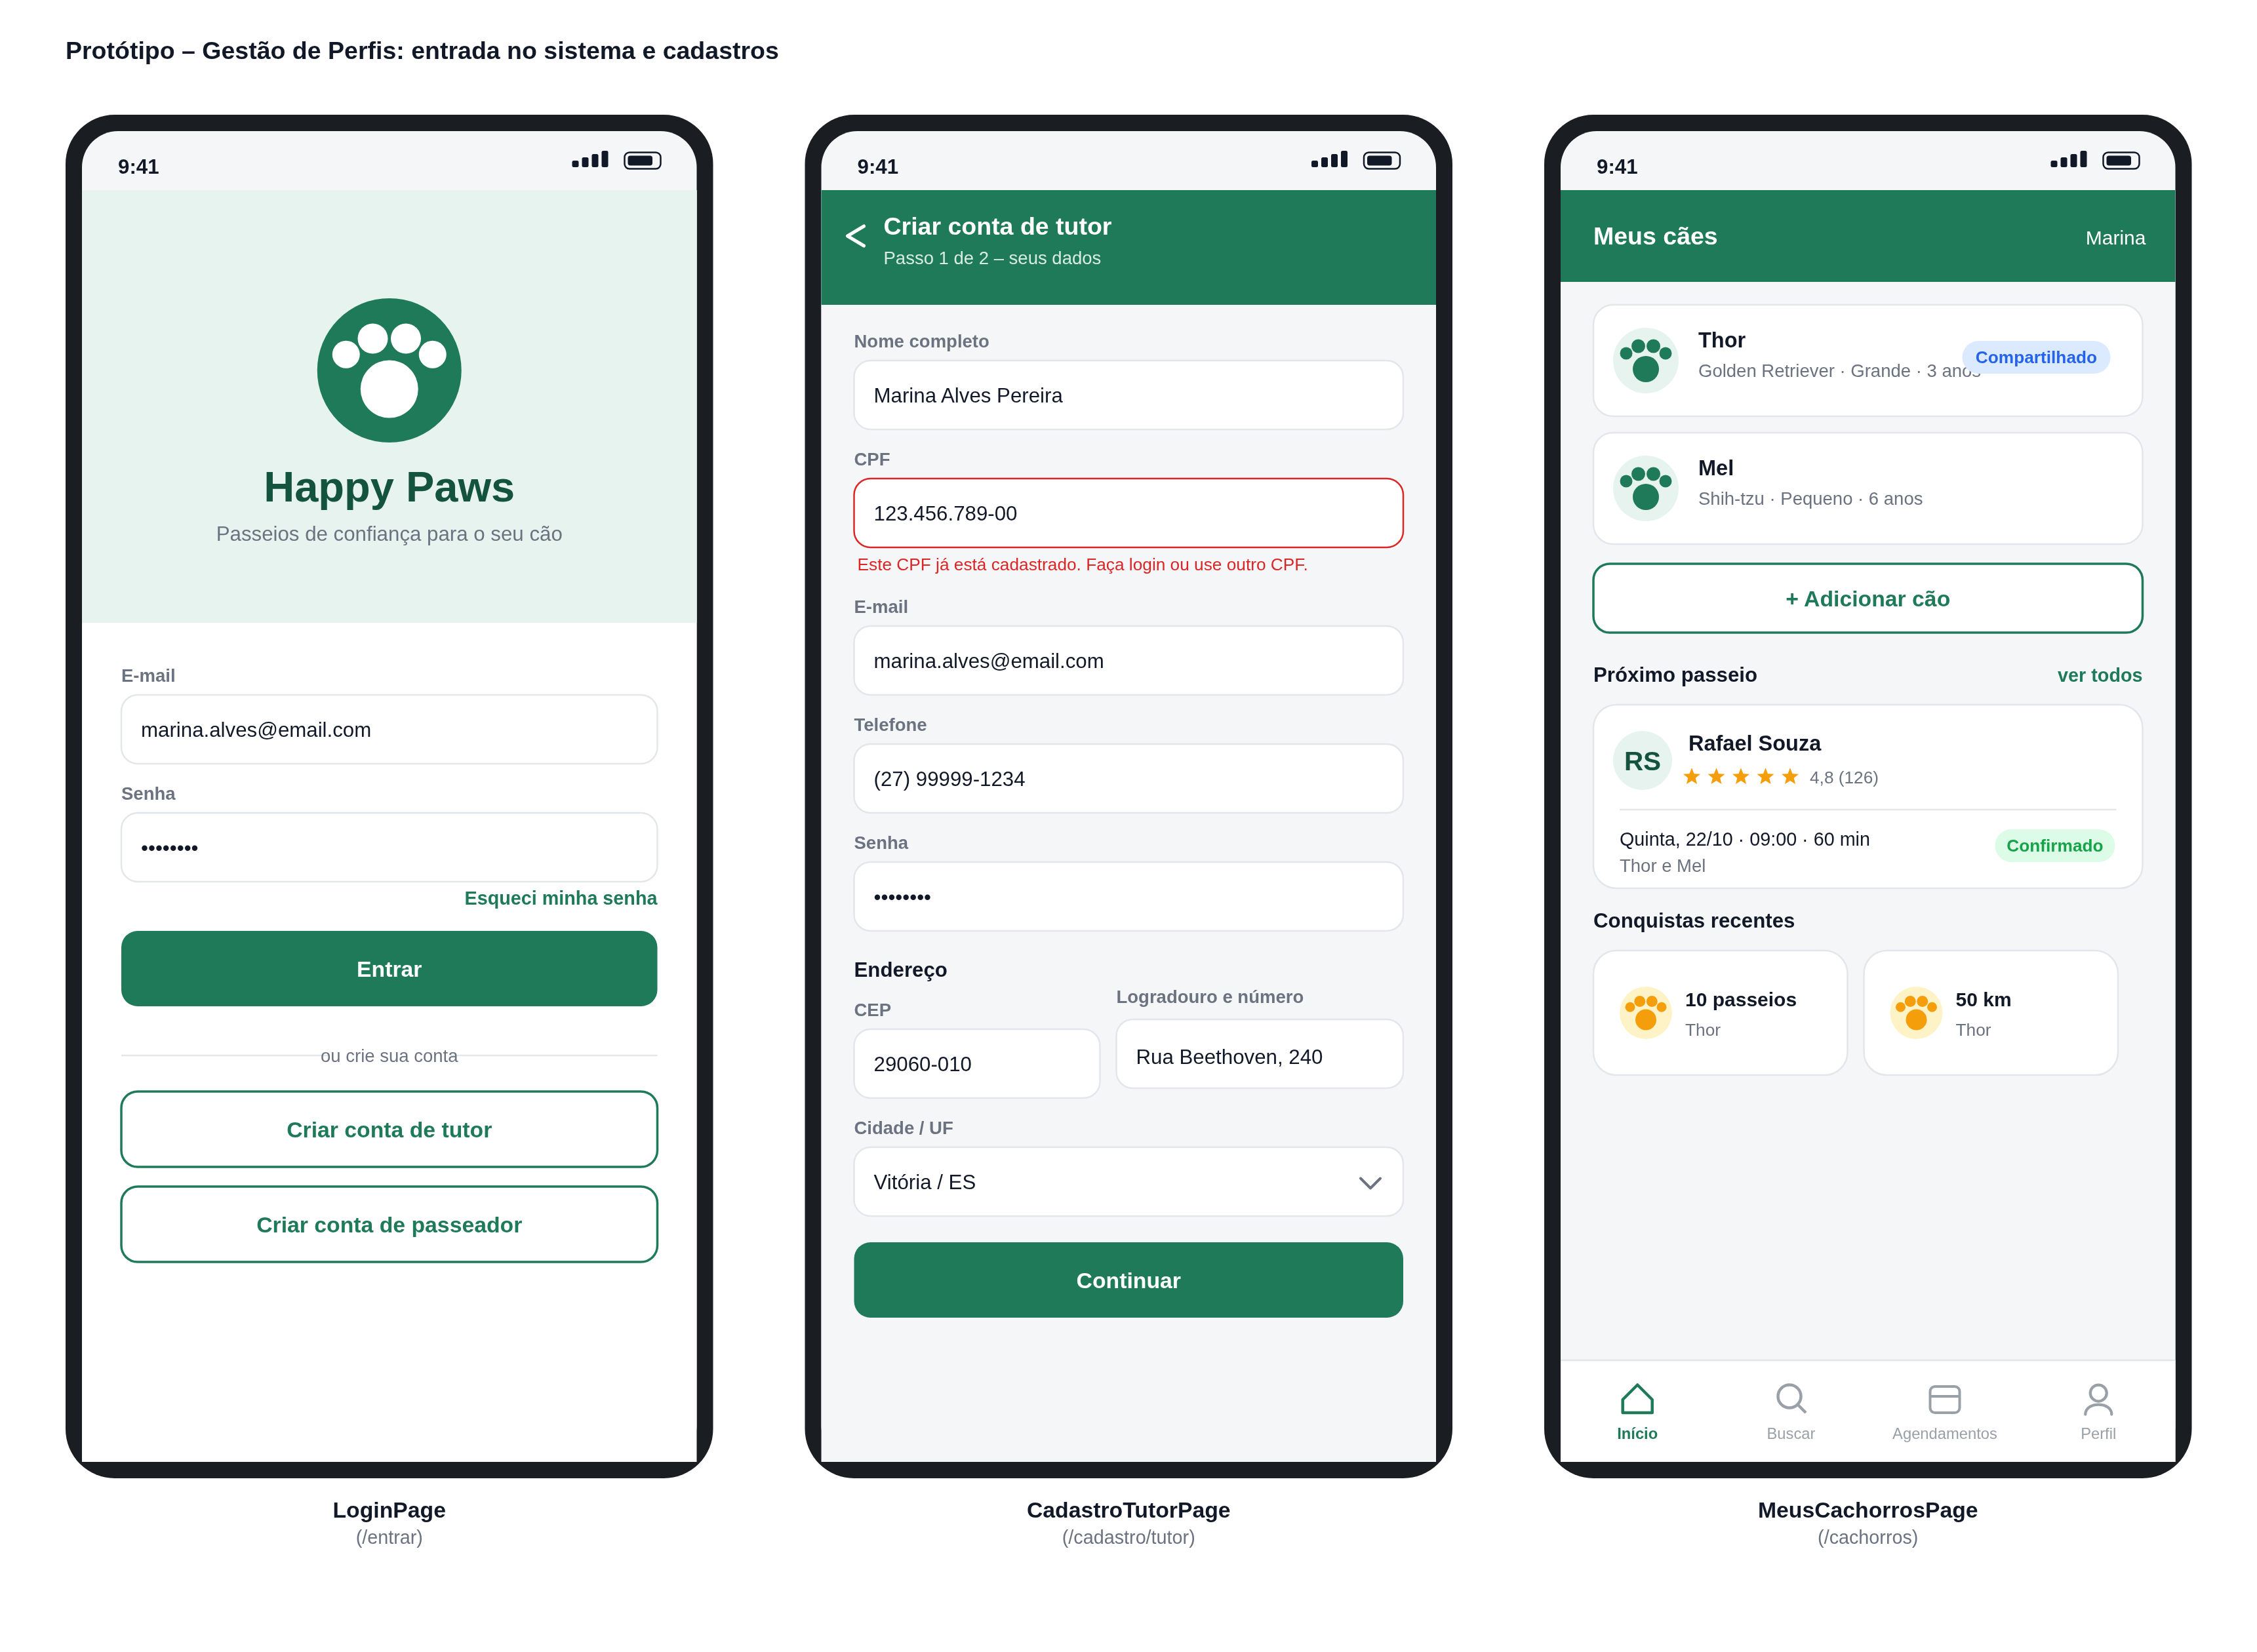
\includegraphics[width=1\textwidth,height=0.85\textheight,keepaspectratio]{figuras/proto-folha-perfis-1.png}
	\caption{Protótipo do subsistema Gestão de Perfis: entrada no sistema e cadastros.}
	\label{figura-proto-perfis-1}
\end{figure}

\begin{figure}[htbp]
	\centering
	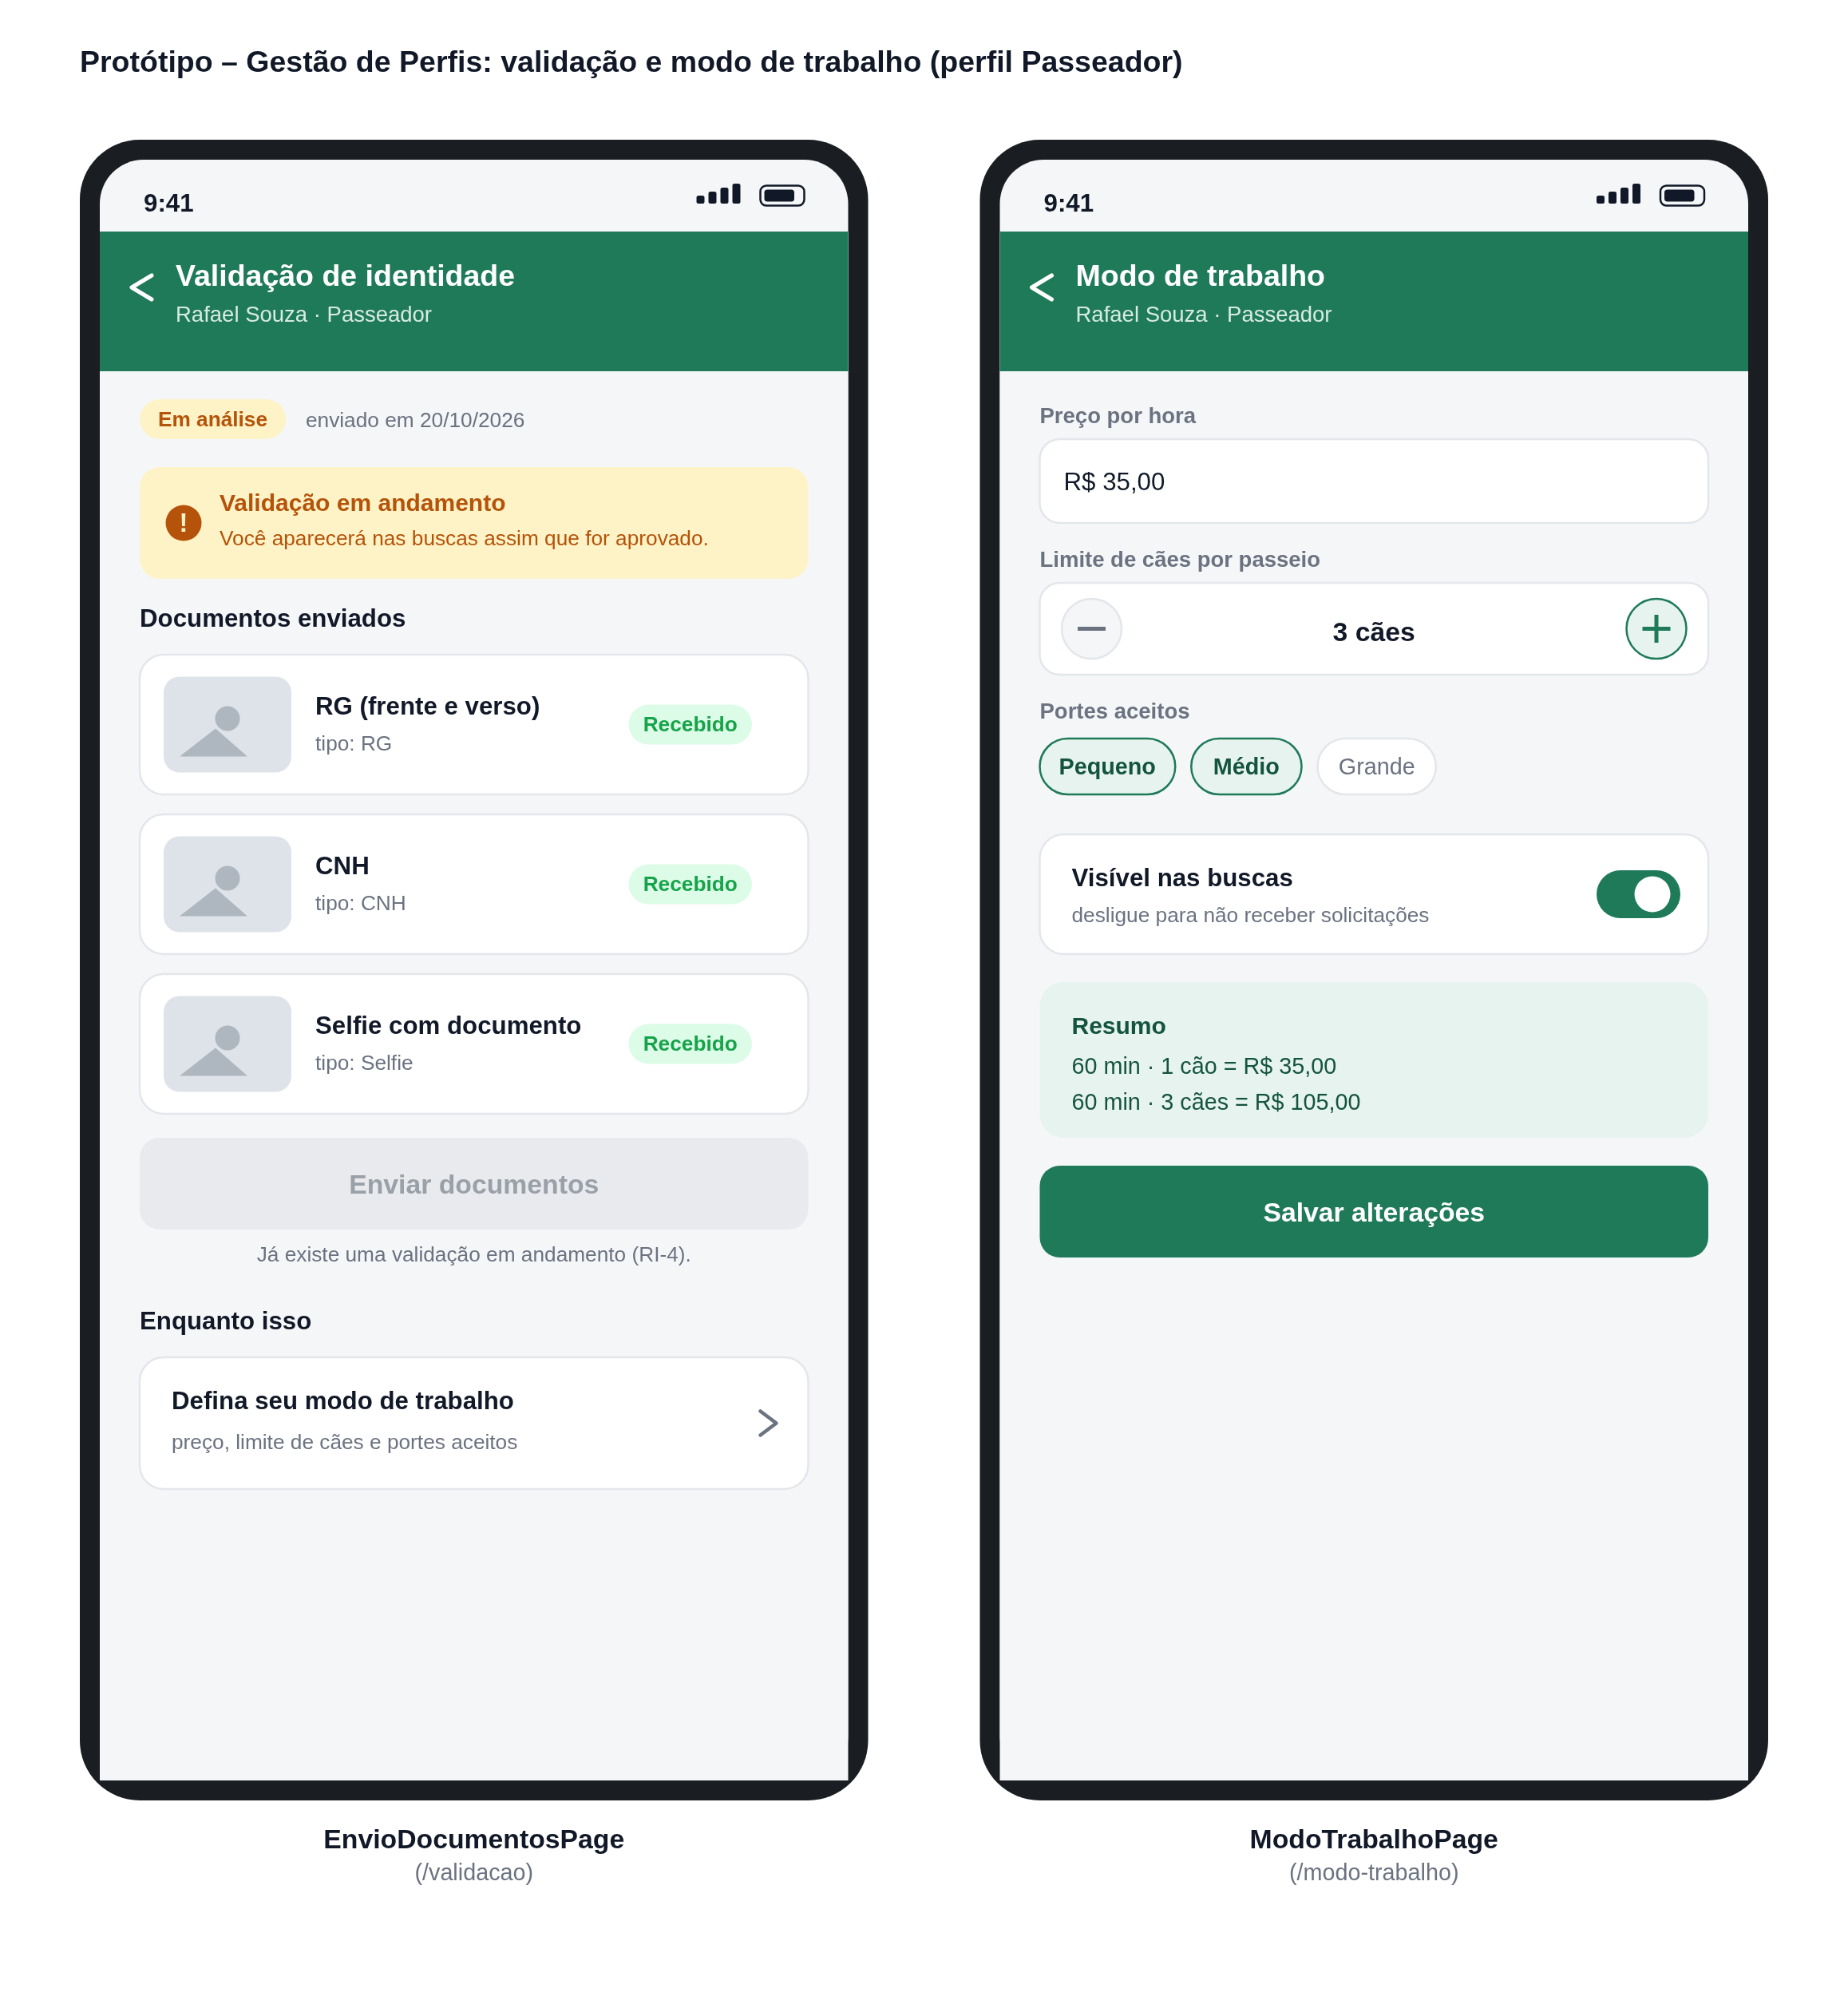
\includegraphics[width=0.68\textwidth,height=0.85\textheight,keepaspectratio]{figuras/proto-folha-perfis-2.png}
	\caption{Protótipo do subsistema Gestão de Perfis: validação de identidade e modo de trabalho (perfil Passeador).}
	\label{figura-proto-perfis-2}
\end{figure}

% ------------------------------------------------------------- Serviços
\begin{figure}[htbp]
	\centering
	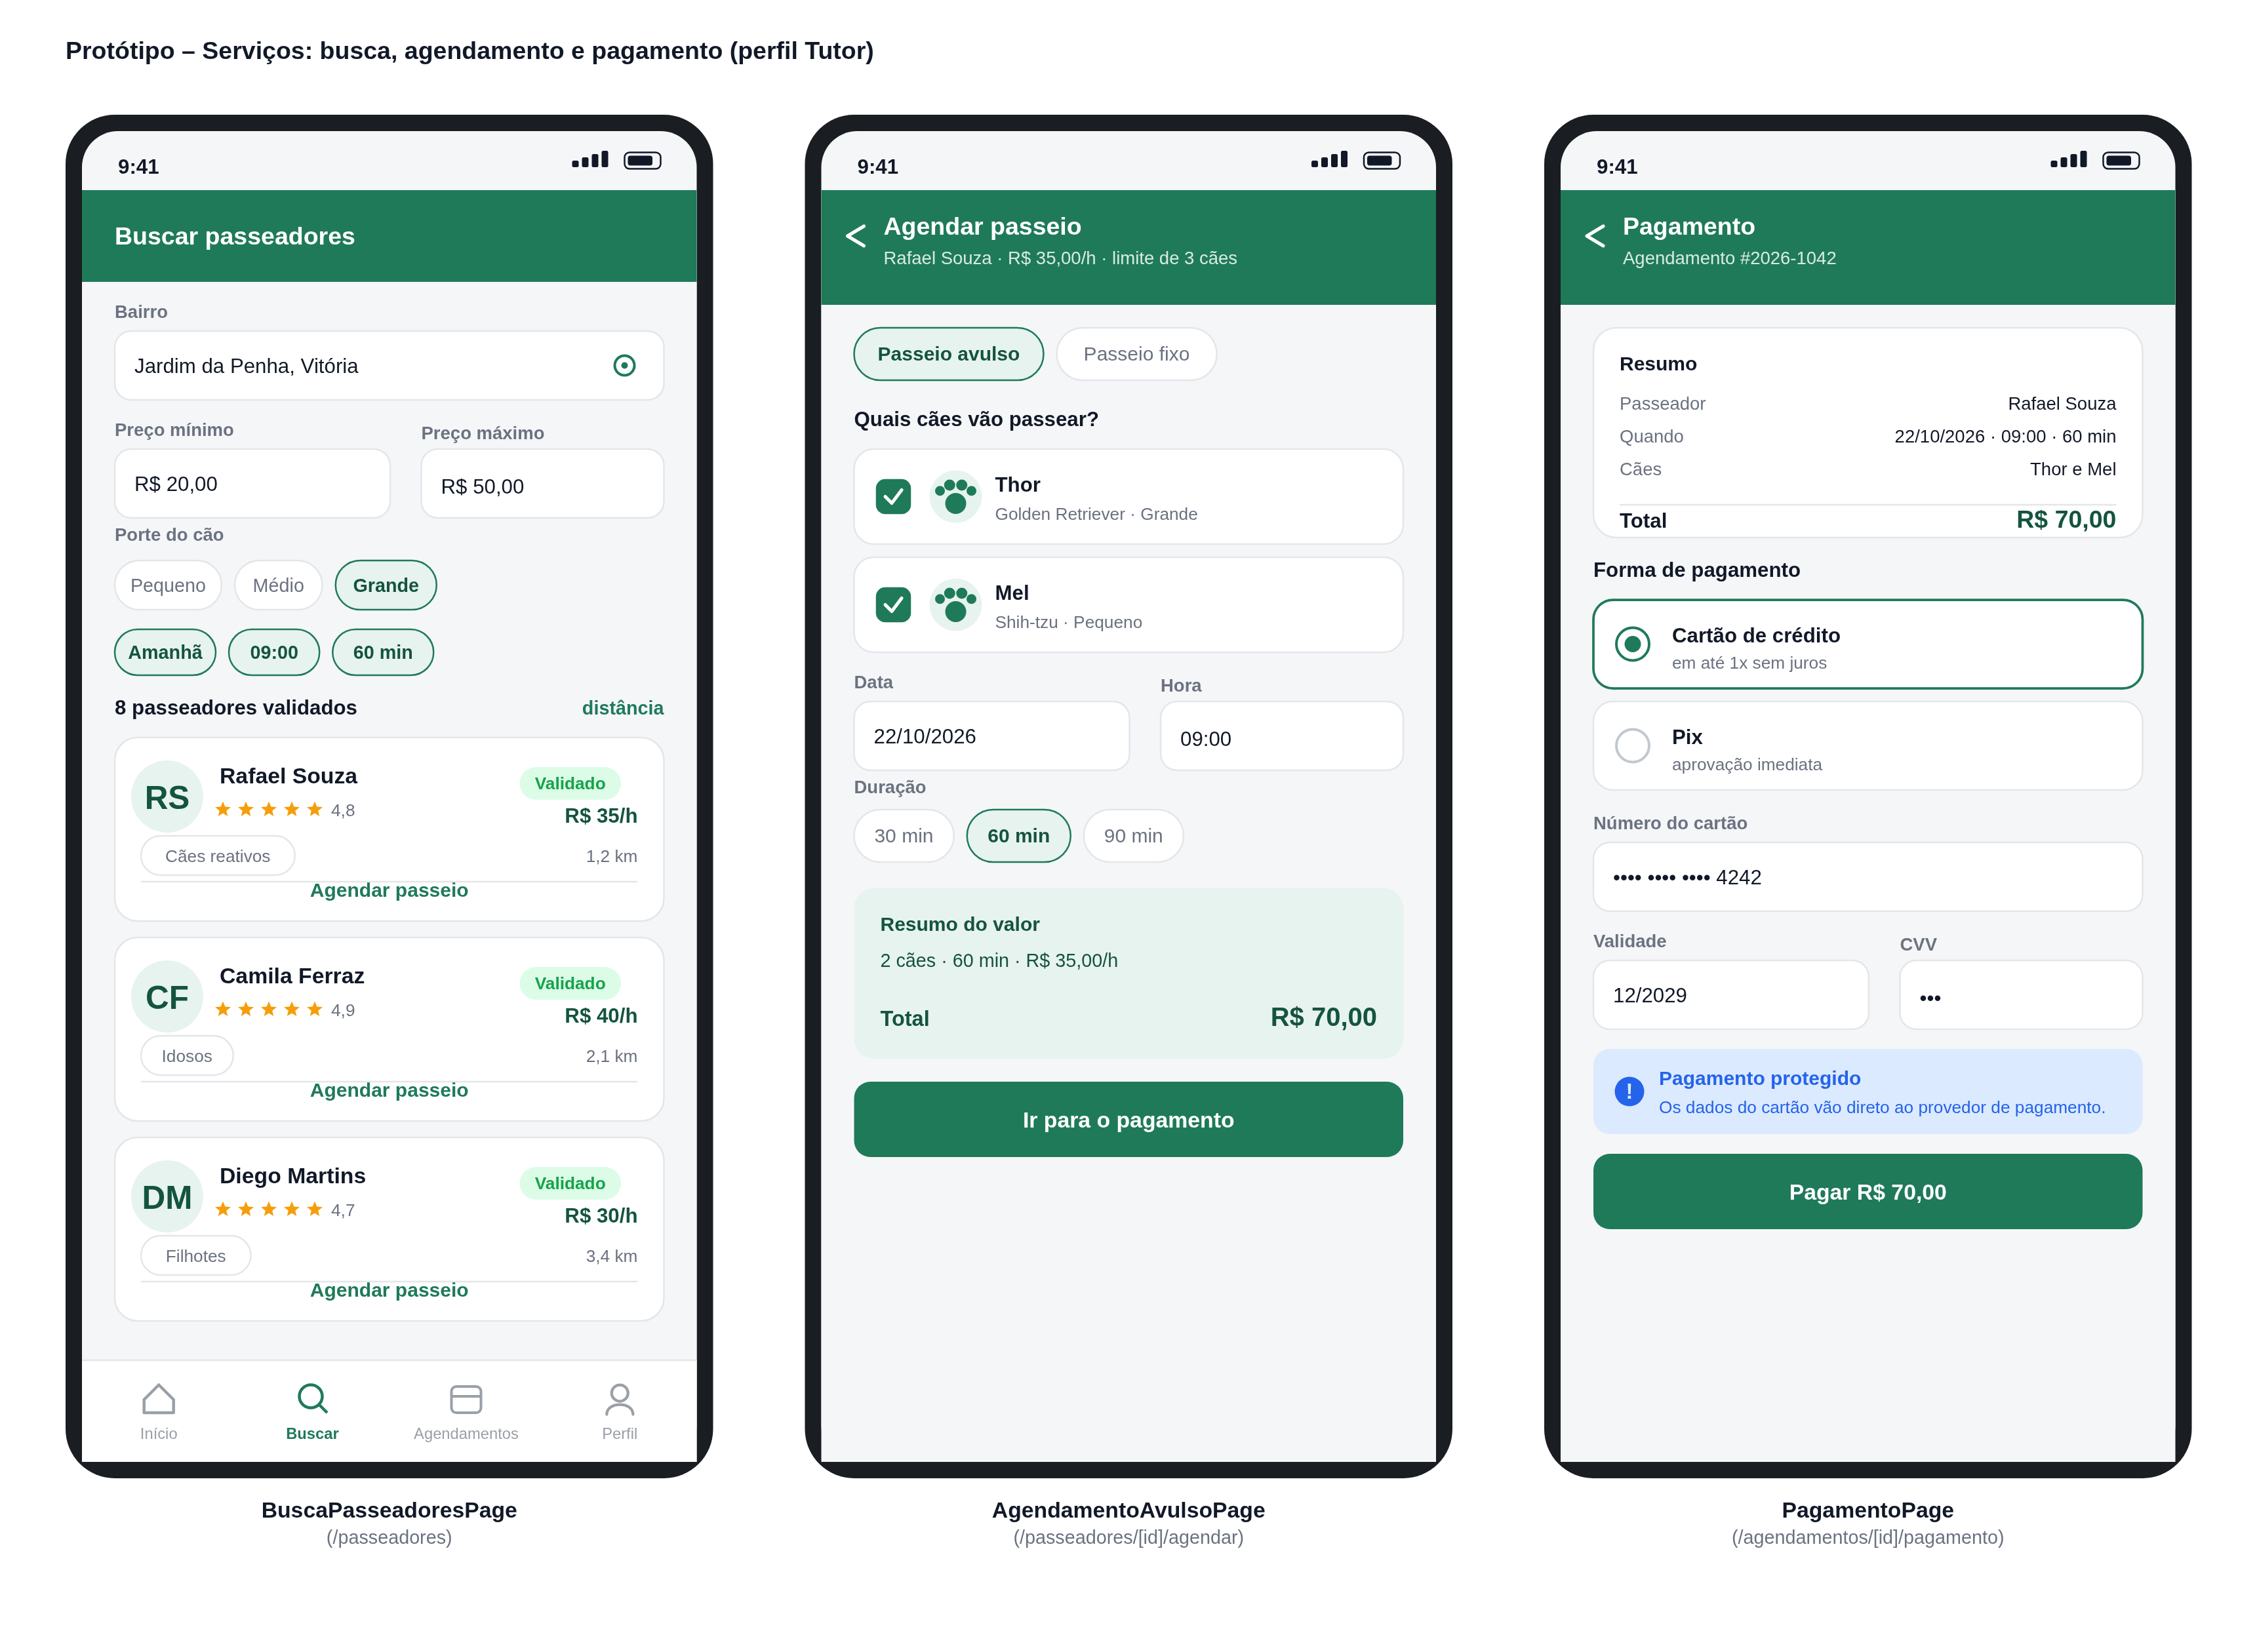
\includegraphics[width=1\textwidth,height=0.85\textheight,keepaspectratio]{figuras/proto-folha-servicos-1.png}
	\caption{Protótipo do subsistema Serviços: busca de passeadores, agendamento e pagamento (perfil Tutor).}
	\label{figura-proto-servicos-1}
\end{figure}

\begin{figure}[htbp]
	\centering
	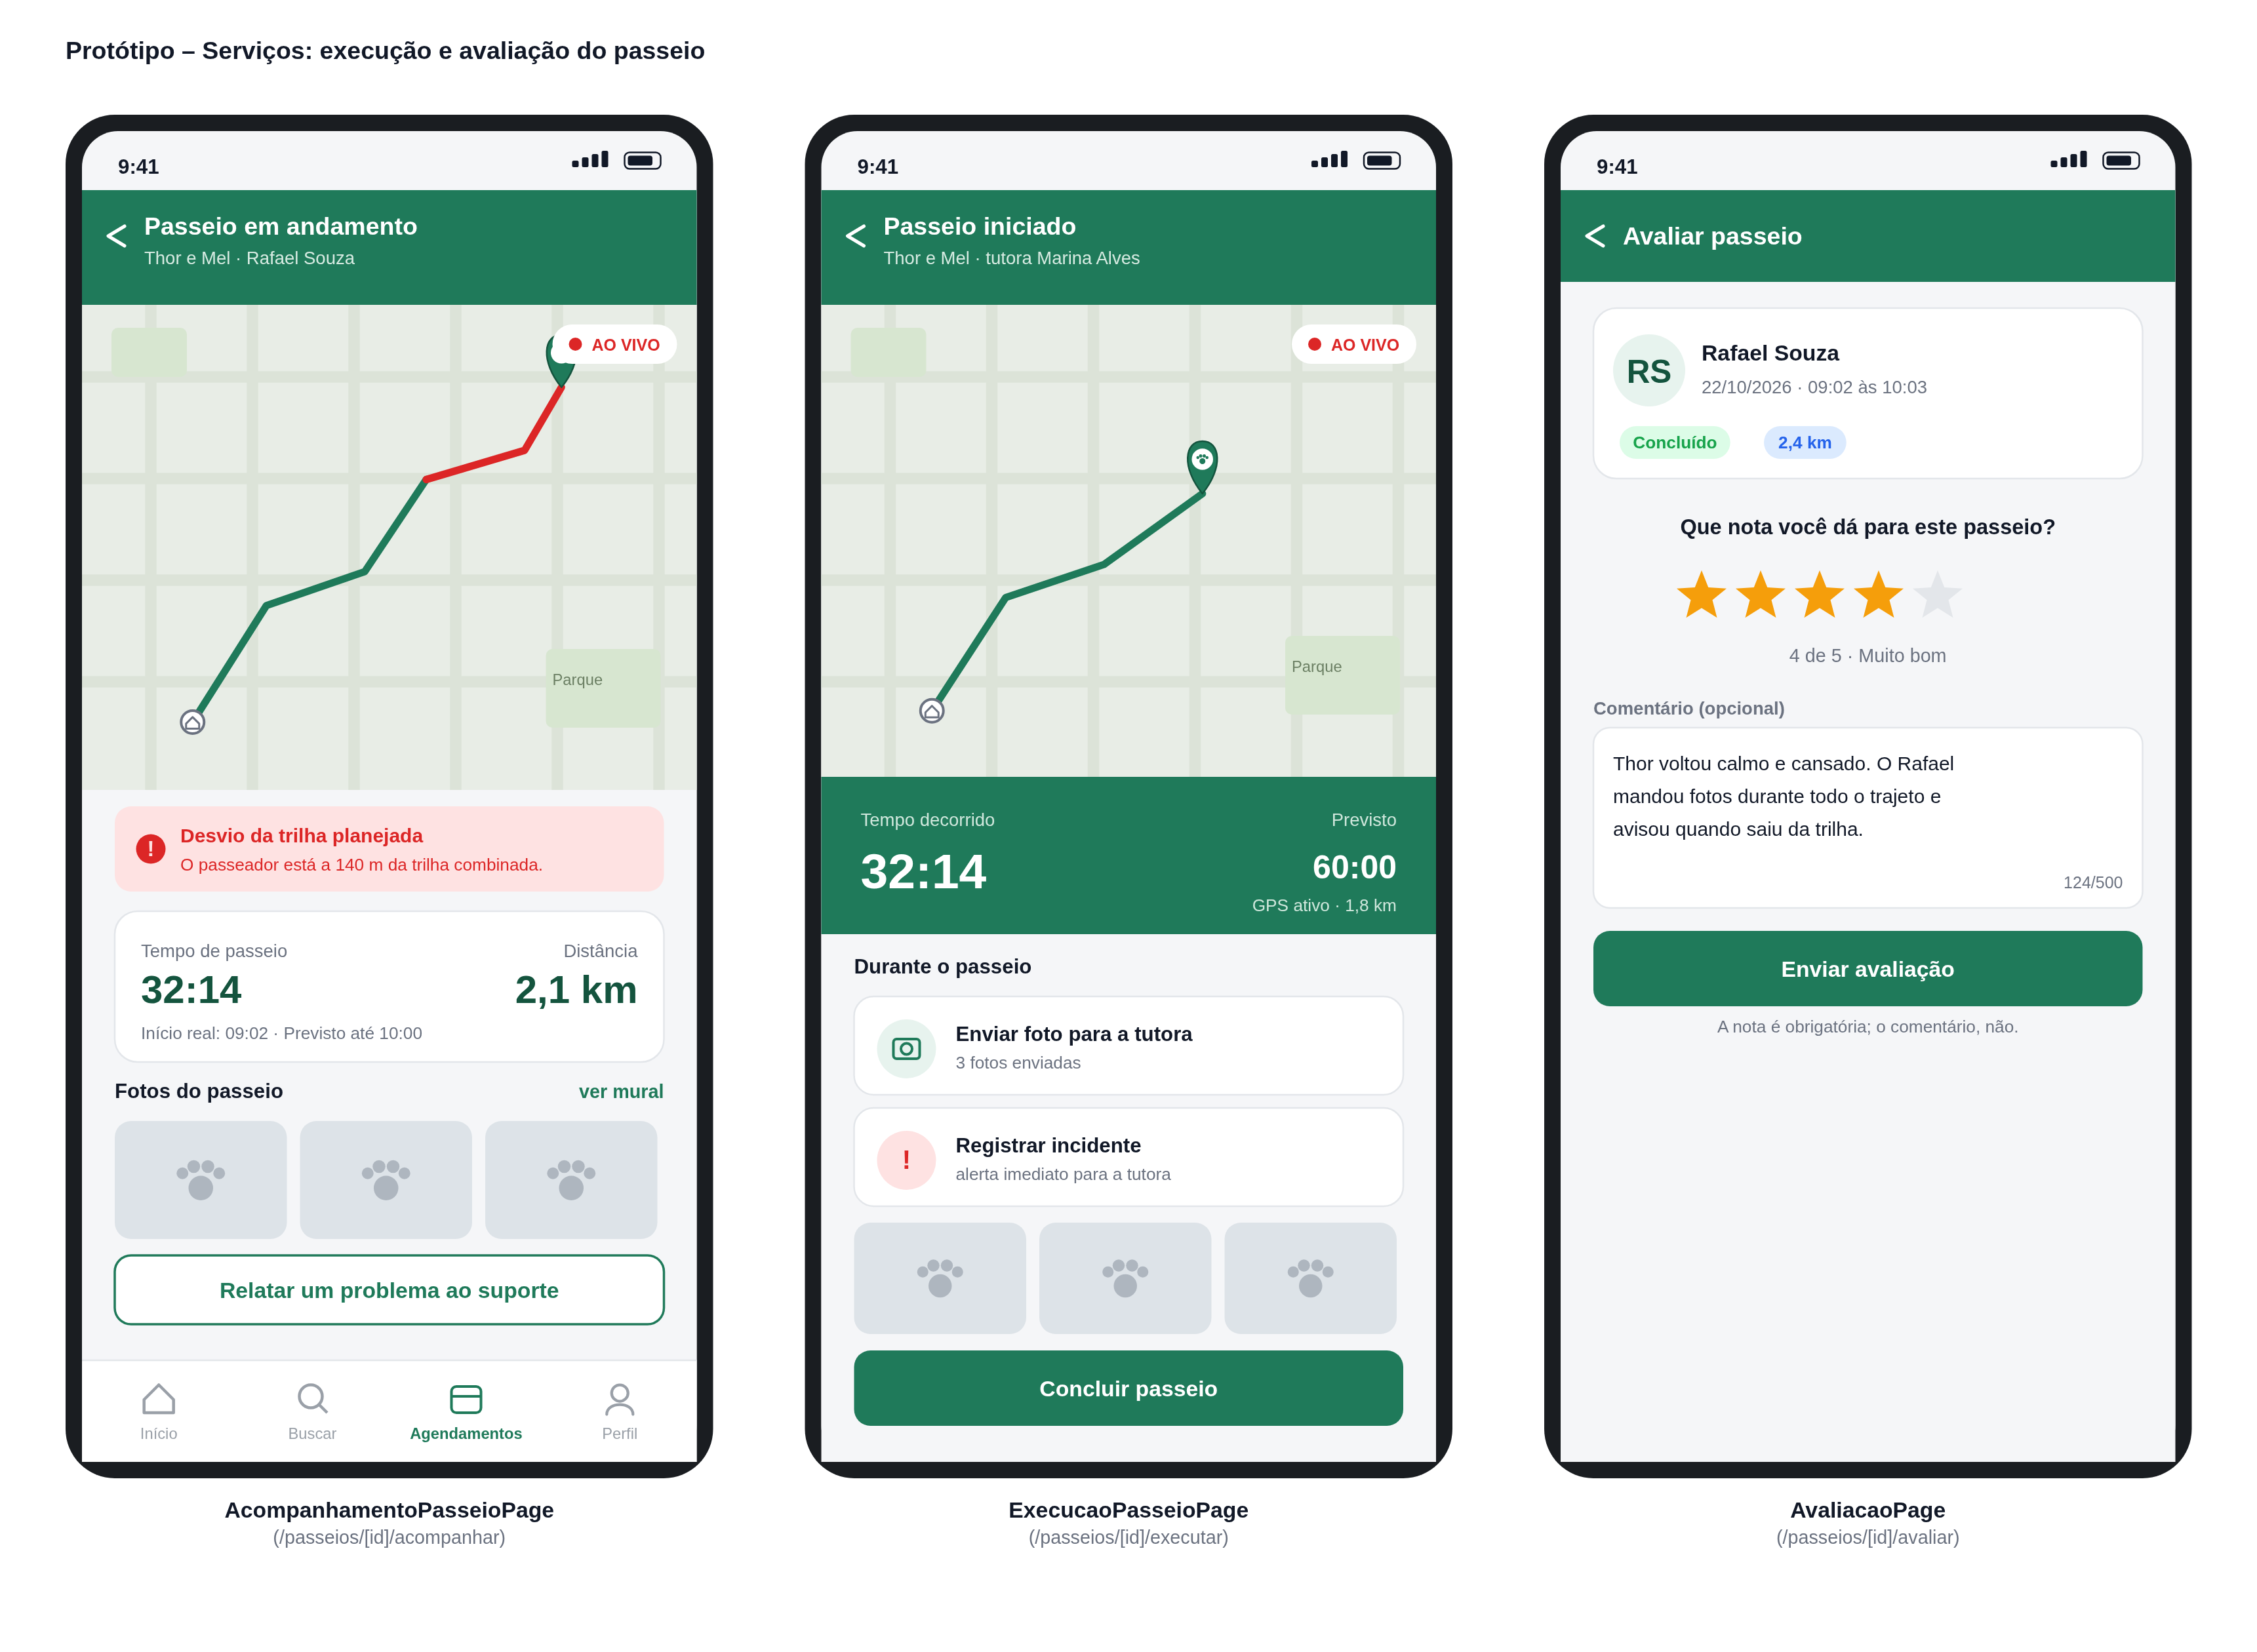
\includegraphics[width=1\textwidth,height=0.85\textheight,keepaspectratio]{figuras/proto-folha-servicos-2.png}
	\caption{Protótipo do subsistema Serviços: acompanhamento em tempo real, execução do passeio e avaliação.}
	\label{figura-proto-servicos-2}
\end{figure}

% -------------------------------------------------------------- Suporte
\begin{figure}[htbp]
	\centering
	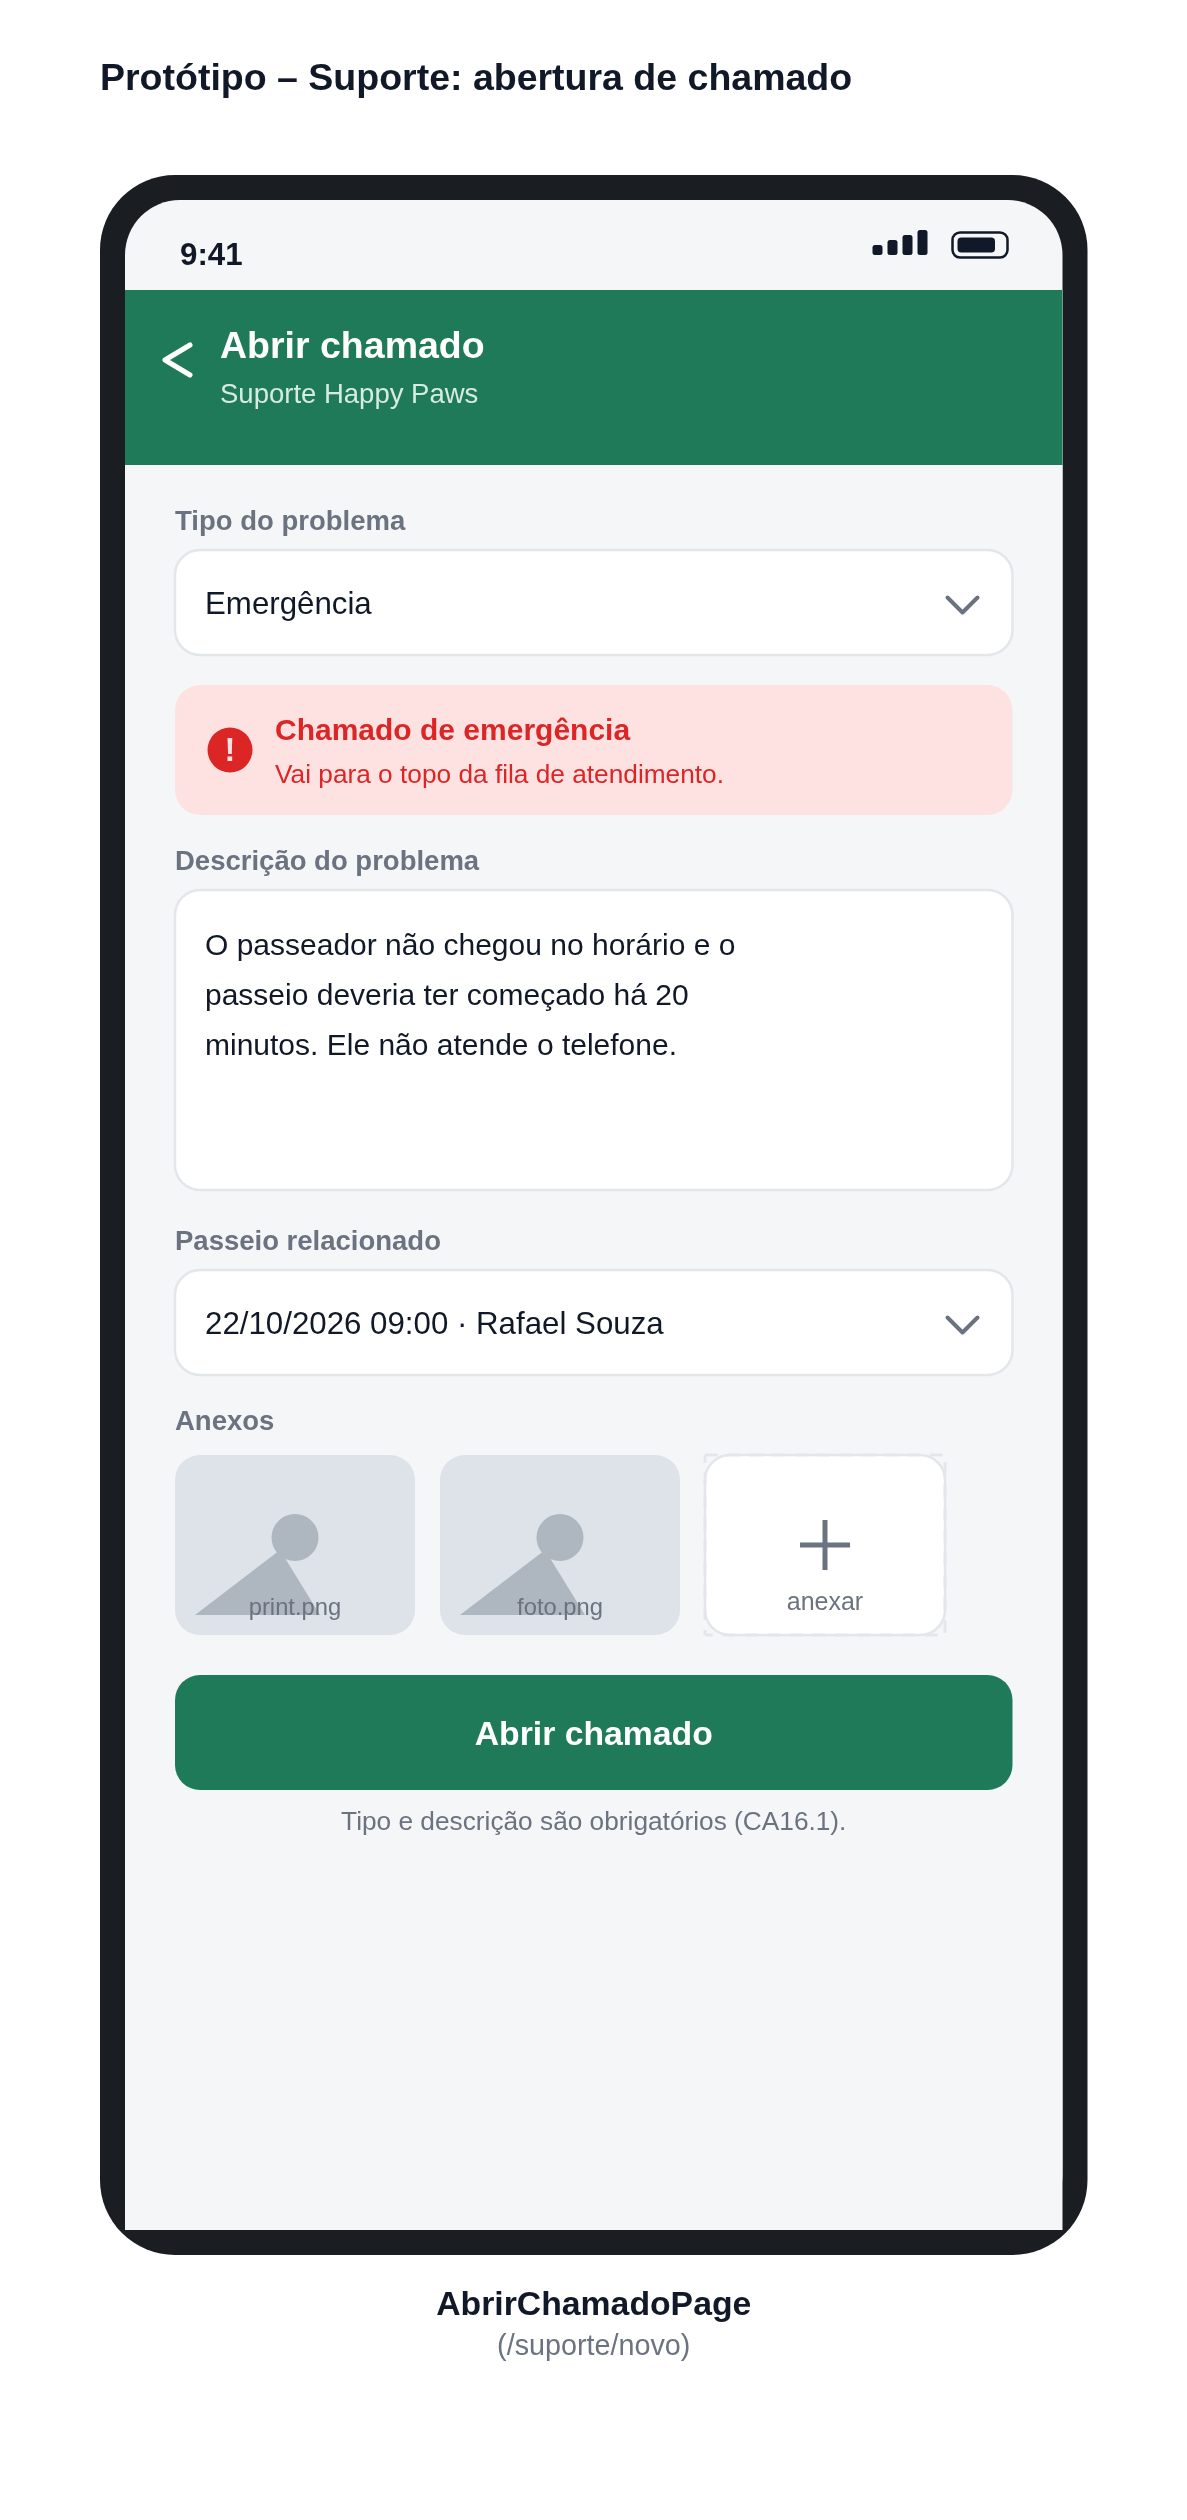
\includegraphics[width=0.29\textwidth,height=0.85\textheight,keepaspectratio]{figuras/proto-folha-suporte.png}
	\caption{Protótipo do subsistema Suporte: abertura de chamado pelo Tutor ou pelo Passeador.}
	\label{figura-proto-suporte}
\end{figure}

\begin{figure}[htbp]
	\centering
	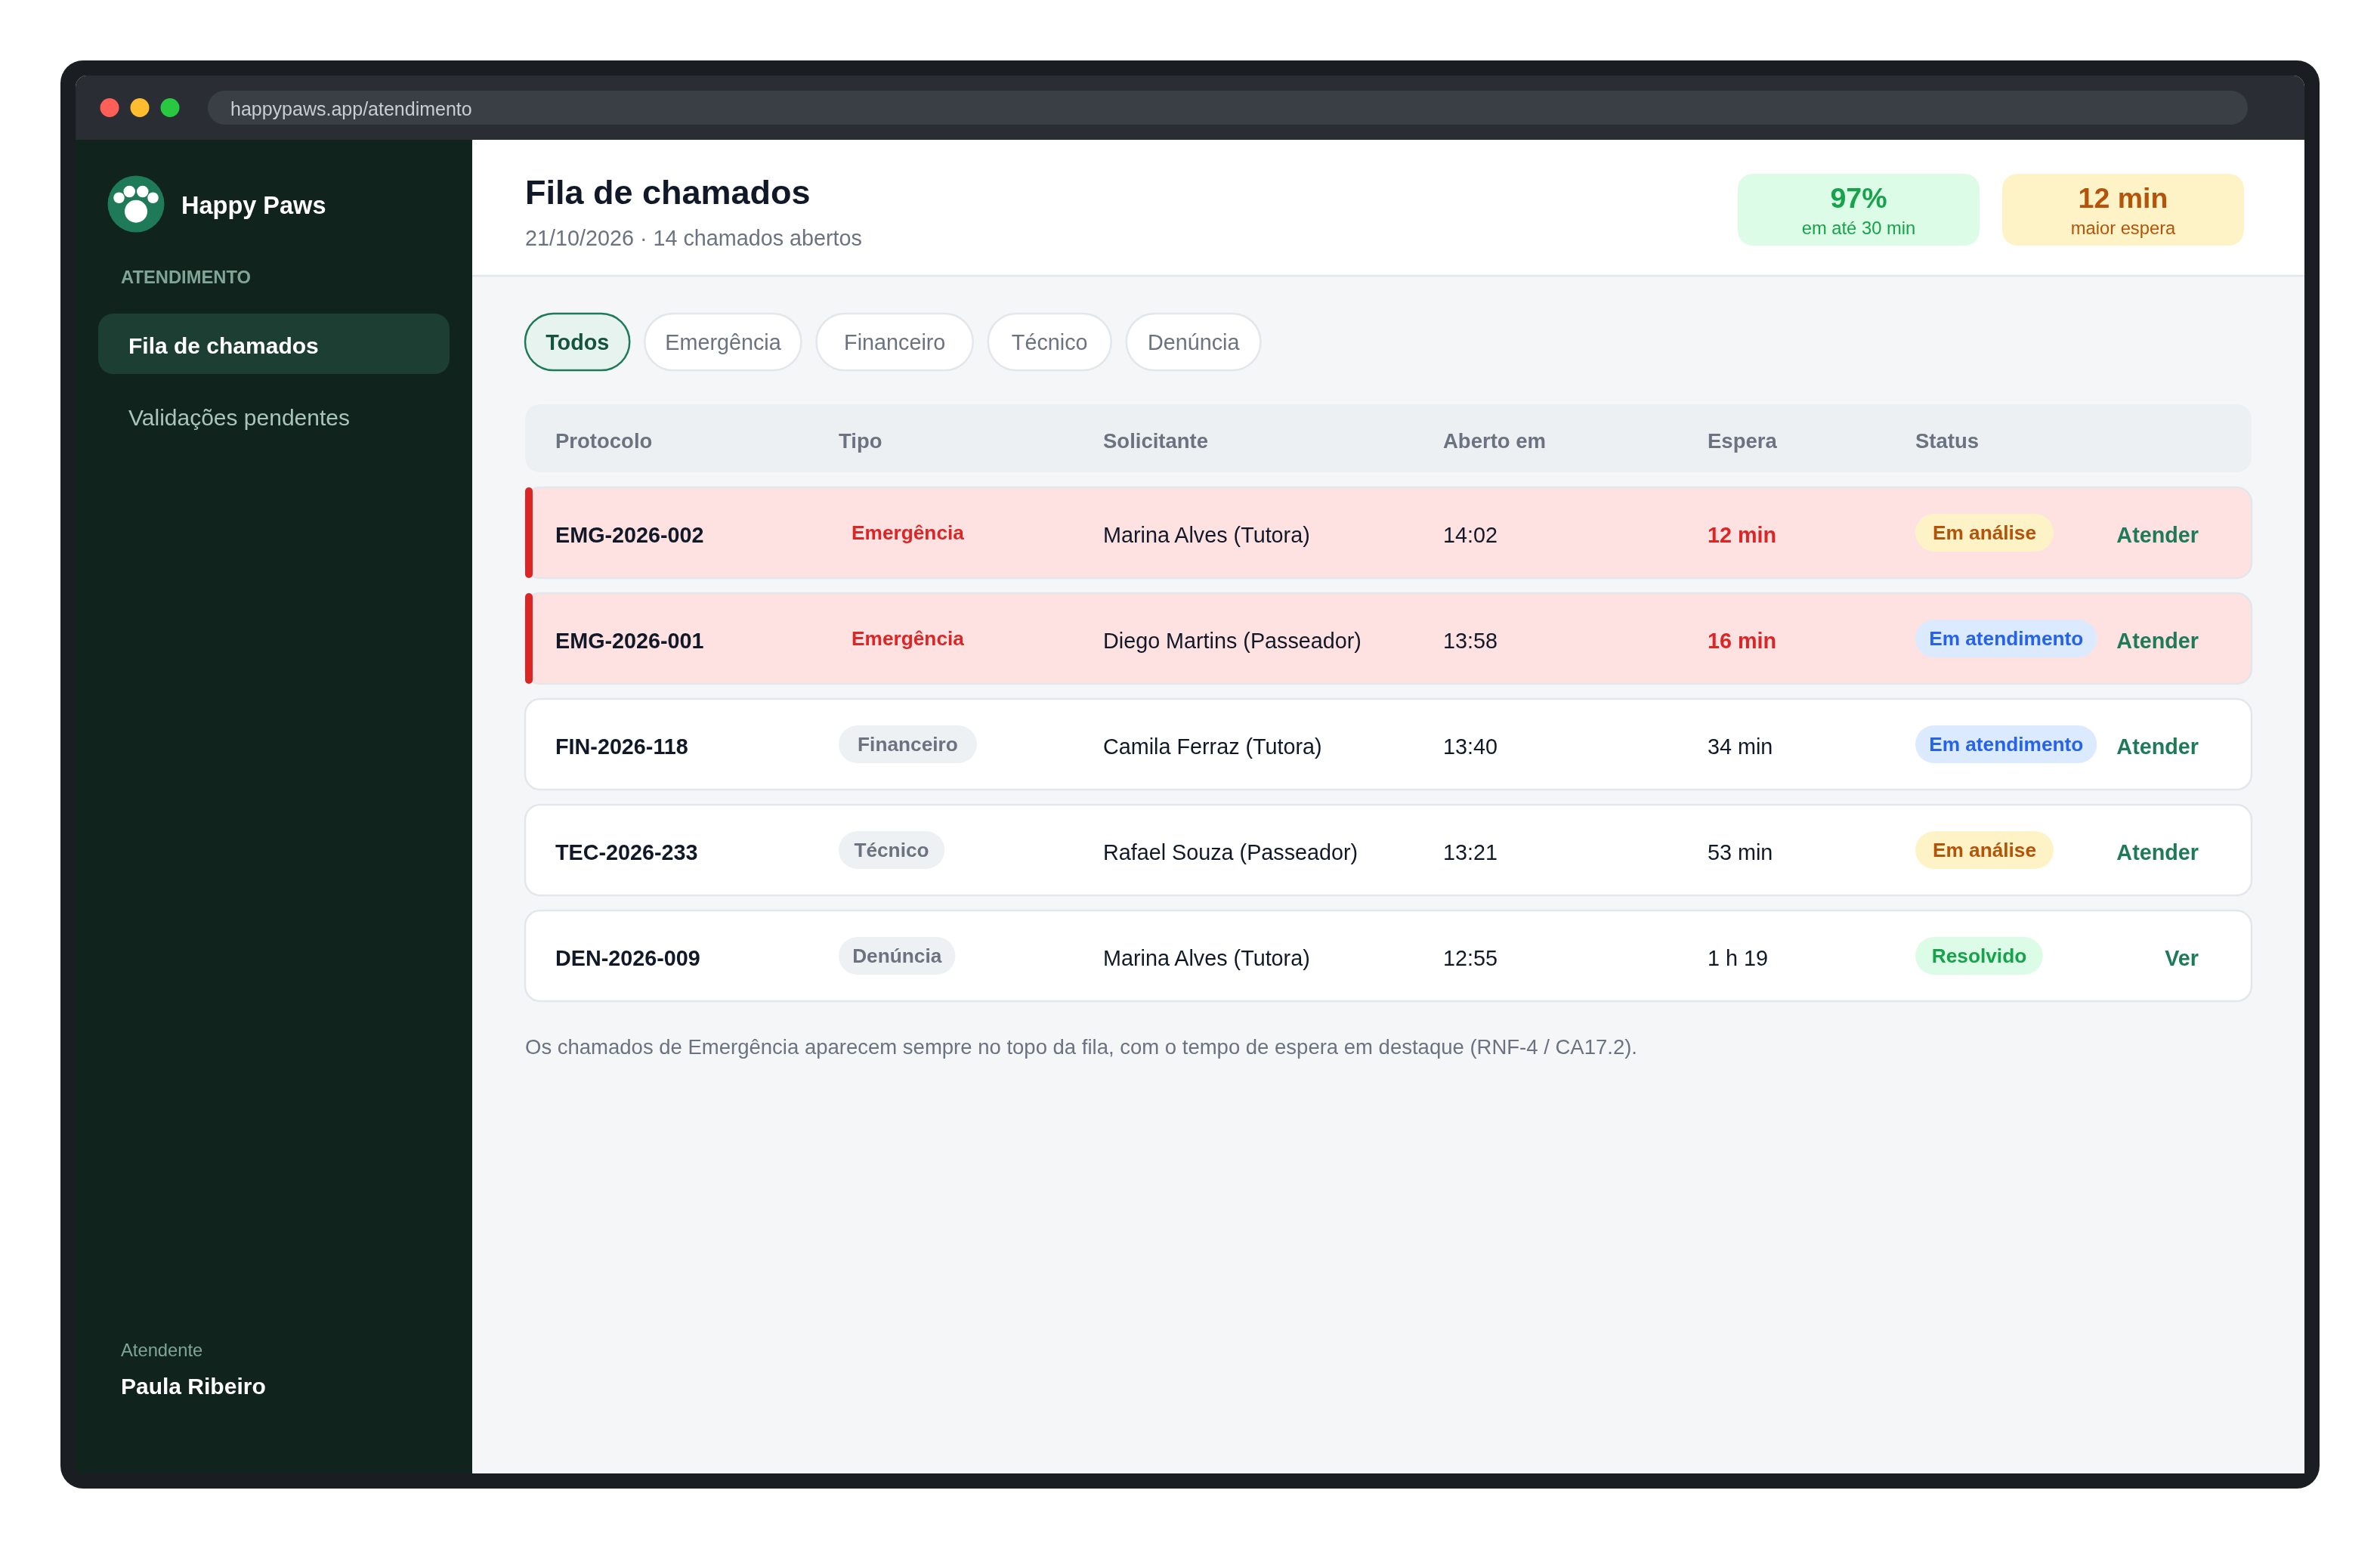
\includegraphics[width=1\textwidth,height=0.85\textheight,keepaspectratio]{figuras/proto-tela-13-fila-atendimento.png}
	\caption{Protótipo da central de atendimento (perfil Atendente): fila de chamados.}
	\label{figura-proto-fila}
\end{figure}

\begin{figure}[htbp]
	\centering
	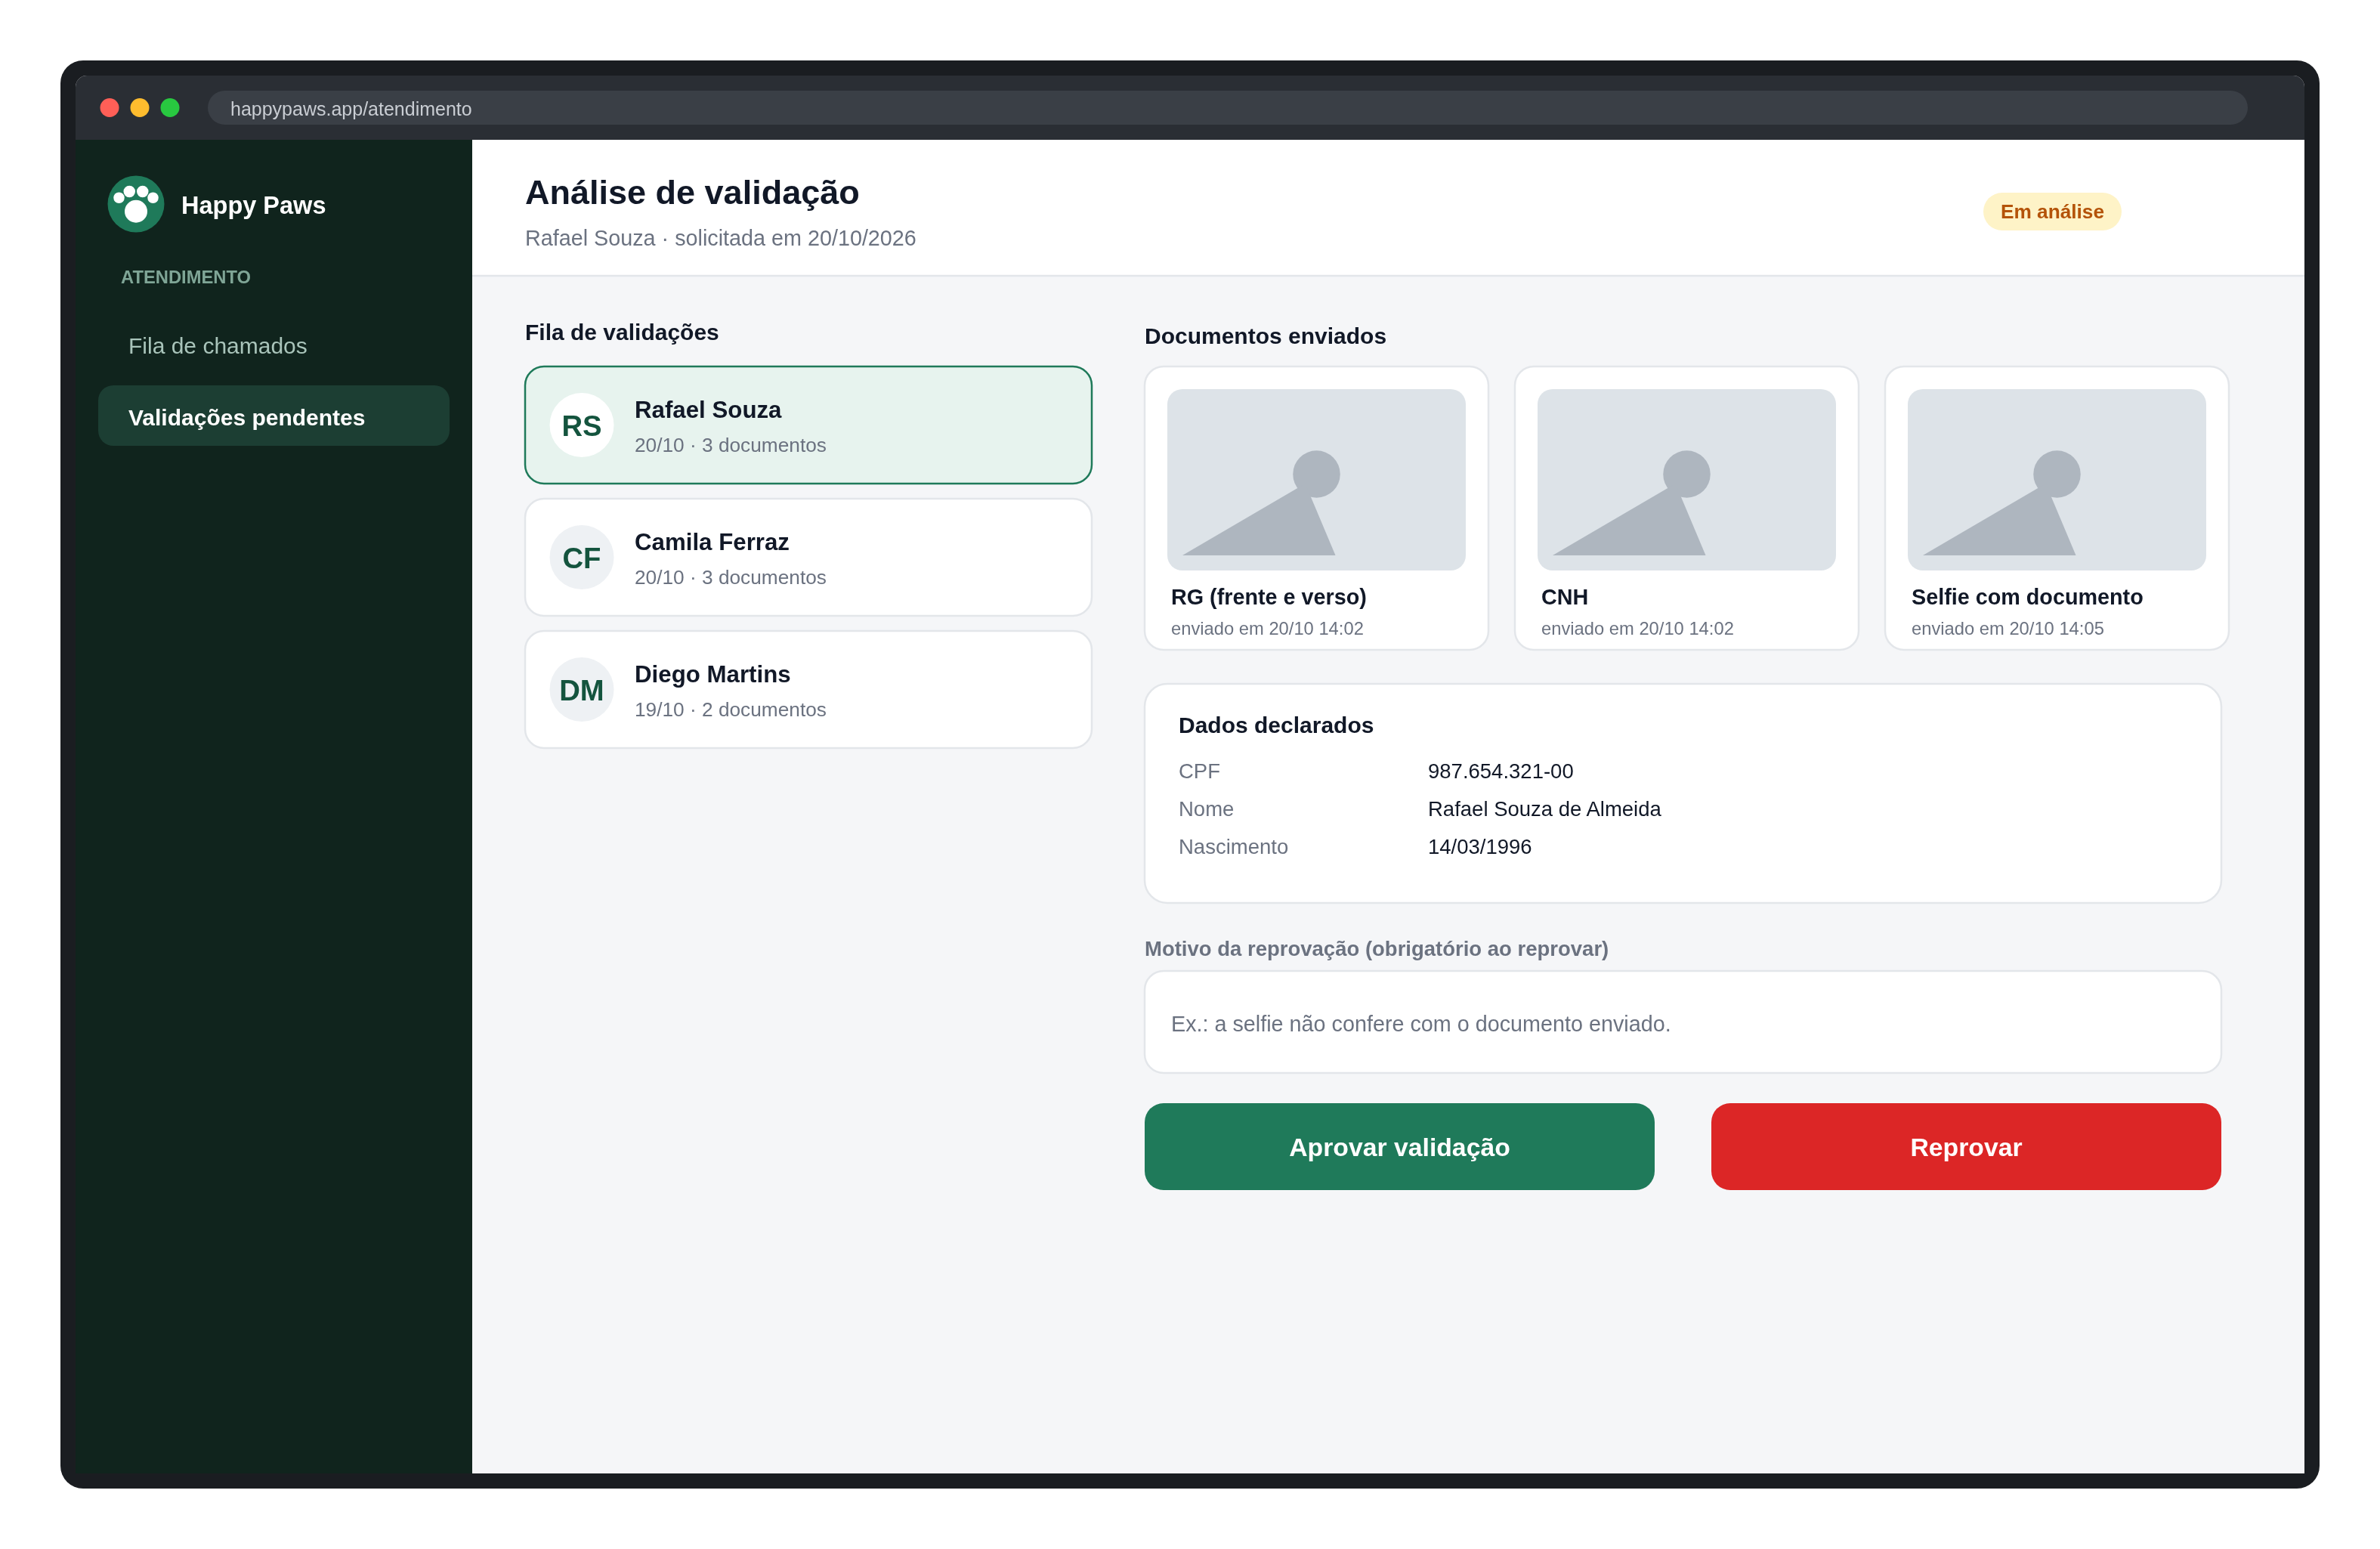
\includegraphics[width=1\textwidth,height=0.85\textheight,keepaspectratio]{figuras/proto-tela-14-analise-validacao.png}
	\caption{Protótipo da central de atendimento (perfil Atendente): análise de validação de identidade do Passeador.}
	\label{figura-proto-validacao}
\end{figure}

As decisões de projeto da interface registradas no protótipo são as seguintes:

\begin{sloppypar}
\begin{itemize}
	\item \textbf{Mensagens de erro junto ao campo.} Em \texttt{CadastroTutorPage} (Figura~\ref{figura-proto-perfis-1}), o erro de CPF já cadastrado (RI-1) aparece abaixo do próprio campo, em linguagem do usuário e com a ação sugerida, e não em uma mensagem genérica no topo da página;

	\item \textbf{Comandos inapropriados desabilitados.} Em \texttt{EnvioDocumentosPage} (Figura~\ref{figura-proto-perfis-2}), o botão de envio fica desabilitado enquanto houver uma validação em andamento (RI-4), e o motivo é informado logo abaixo do botão. A mesma tática vale para o botão ``Iniciar passeio'', que só é habilitado com o pagamento confirmado (CA14.5);

	\item \textbf{Entrada por seleção.} Porte, especialidades, portes aceitos, duração, tipo de agendamento, método de pagamento, tipo de documento e tipo de chamado são escolhidos em listas, botões de opção ou \textit{chips}, nunca digitados (Tabela~\ref{tabela-enumerados}); a localização da busca é obtida pela \textit{Geolocation API} e os cães do agendamento vêm da lista de cães do próprio Tutor;

	\item \textbf{Resumo antes do compromisso.} As telas de agendamento e de pagamento (Figura~\ref{figura-proto-servicos-1}) mostram o valor calculado por \texttt{Agendamento.calcularValor()} antes de o Tutor confirmar, e a tela de pagamento informa que os dados do cartão são enviados diretamente ao provedor de pagamento (RNF-2);

	\item \textbf{Estado do sistema sempre visível.} A tela de acompanhamento (Figura~\ref{figura-proto-servicos-2}) tem o indicador ``AO VIVO'', o tempo decorrido, a distância percorrida e o aviso de desvio de rota em destaque; o trecho fora da trilha planejada aparece em vermelho no mapa (CA10.3);

	\item \textbf{Telas de uso em movimento.} A tela de execução do passeio (perfil Passeador) usa poucos comandos, botões grandes, alto contraste e nenhuma digitação obrigatória: o cronômetro e os comandos de foto, de incidente e de conclusão ocupam toda a largura da tela;

	\item \textbf{Iniciativa do sistema na fila de atendimento.} Em \texttt{FilaAtendimentoPage} (Figura~\ref{figura-proto-fila}), os chamados do tipo ``Emergência'' aparecem no topo, com faixa e tempo de espera em destaque, e o indicador de primeiro atendimento em até 30 minutos fica no cabeçalho (RNF-4 e CA17.2);

	\item \textbf{Dados obrigatórios no momento certo.} Na análise de validação (Figura~\ref{figura-proto-validacao}), o campo de motivo fica junto dos botões e é obrigatório apenas quando o Atendente reprova a validação (CA04.4); na avaliação do passeio, a nota é obrigatória e o comentário é opcional.
\end{itemize}
\end{sloppypar}

Em relação ao protótipo de Engenharia de Software I, esta versão acrescenta as telas do perfil Atendente (fila de chamados e análise de validação), separa as páginas por rota e por perfil, conforme as Tabelas~\ref{tabela-ciu-perfis} a~\ref{tabela-ciu-suporte}, e incorpora as táticas de usabilidade da Tabela~\ref{tabela-taticas-usabilidade}.

O protótipo completo desta revisão pode ser visto na Web em \url{https://raw.githack.com/Eduardo-Ferraz/happy-paws-go/main/docs/es2-projeto/prototipo/index.html}. Os arquivos ficam no repositório do projeto, em \url{https://github.com/Eduardo-Ferraz/happy-paws-go/tree/main/docs/es2-projeto/prototipo}, em formato vetorial (SVG), uma tela por arquivo, nomeadas pela página correspondente do pacote \texttt{cih}.
